%==============================================================================
% Figure: G2 Root System
% Purpose: Visualize G2 exceptional Lie algebra root structure
% Chapter: Ch03 - Exceptional Lie Groups
% Type: Mathematical
%==============================================================================

\begin{figure}[htbp]
  \centering
  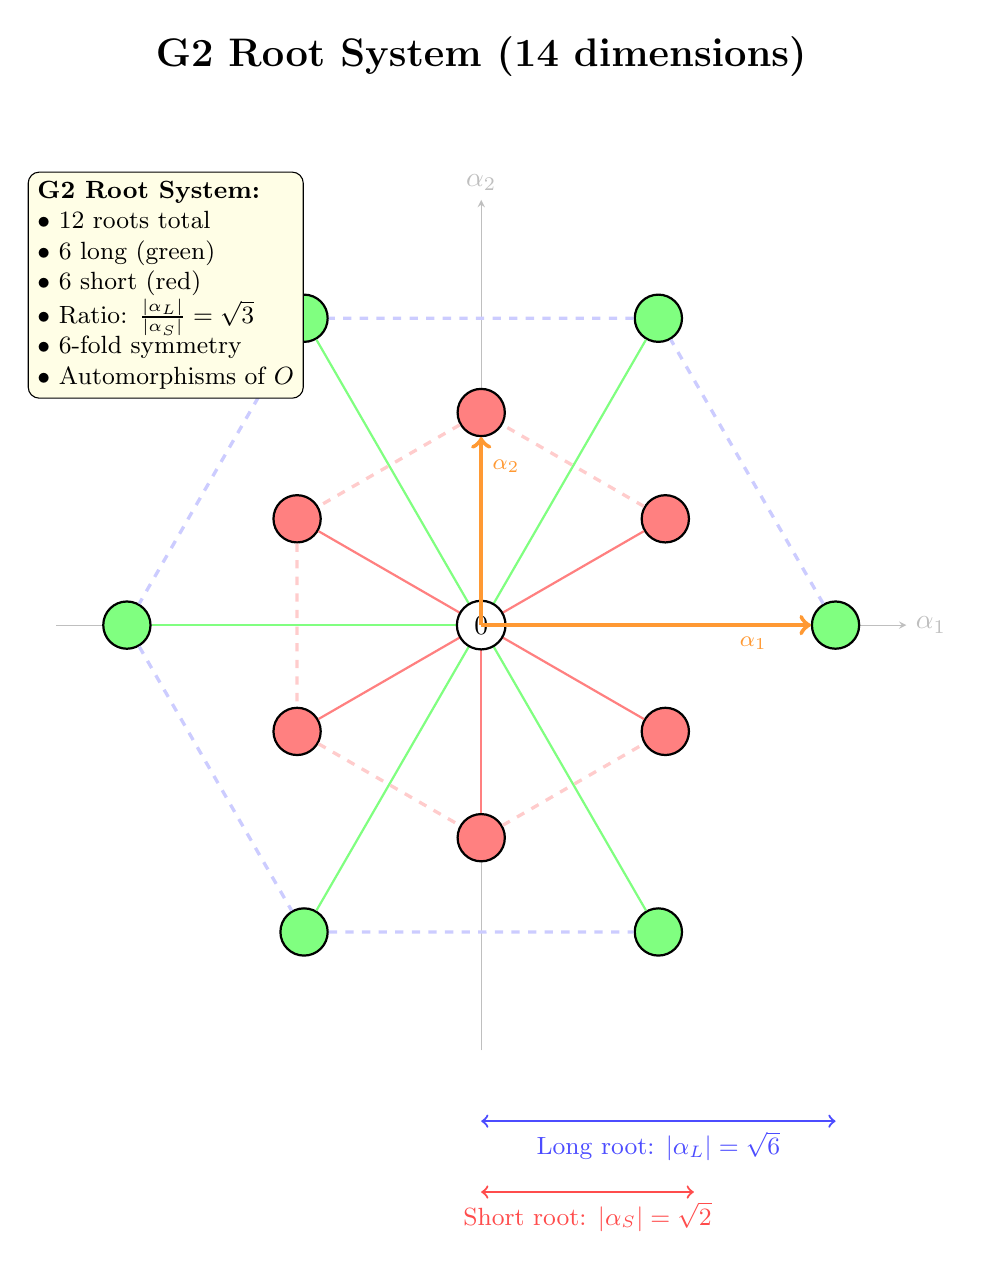
\begin{tikzpicture}[
    scale=1.8,
    root/.style={circle, draw=black, fill=blue!30, thick, minimum size=5mm},
    short_root/.style={circle, draw=black, fill=red!50, thick, minimum size=6mm},
    long_root/.style={circle, draw=black, fill=green!50, thick, minimum size=6mm},
    arrow/.style={->, >=stealth, thick, gray!50}
  ]

    % G2 has 12 roots (6 long, 6 short) in a hexagonal pattern
    % Long roots at 60-degree intervals
    % Short roots at 60-degree intervals, rotated 30 degrees

    \def\longradius{2.5}
    \def\shortradius{1.5}

    % Draw coordinate axes
    \draw[arrow, very thin] (-3, 0) -- (3, 0) node[right] {$\alpha_1$};
    \draw[arrow, very thin] (0, -3) -- (0, 3) node[above] {$\alpha_2$};

    % Long roots (6 roots at 60-degree intervals)
    \foreach \i in {0, 1, 2, 3, 4, 5} {
      \pgfmathsetmacro\angle{60 * \i}
      \pgfmathsetmacro\x{\longradius * cos(\angle)}
      \pgfmathsetmacro\y{\longradius * sin(\angle)}
      \node[long_root] (L\i) at (\x, \y) {};
      \draw[green!50, thick] (0, 0) -- (L\i);
    }

    % Short roots (6 roots at 60-degree intervals, rotated 30 degrees)
    \foreach \i in {0, 1, 2, 3, 4, 5} {
      \pgfmathsetmacro\angle{60 * \i + 30}
      \pgfmathsetmacro\x{\shortradius * cos(\angle)}
      \pgfmathsetmacro\y{\shortradius * sin(\angle)}
      \node[short_root] (S\i) at (\x, \y) {};
      \draw[red!50, thick] (0, 0) -- (S\i);
    }

    % Origin
    \node[circle, draw=black, fill=white, thick, minimum size=4mm] at (0, 0) {$0$};

    % Highlight hexagonal symmetry with faint hexagon
    \draw[blue!20, very thick, dashed]
      (L0) -- (L1) -- (L2) -- (L3) -- (L4) -- (L5) -- cycle;
    \draw[red!20, very thick, dashed]
      (S0) -- (S1) -- (S2) -- (S3) -- (S4) -- (S5) -- cycle;

    % Annotations for root lengths
    \draw[<->, thick, blue!70] (0, -3.5) -- (\longradius, -3.5)
      node[midway, below, font=\small] {Long root: $|\alpha_L| = \sqrt{6}$};
    \draw[<->, thick, red!70] (0, -4.0) -- (\shortradius, -4.0)
      node[midway, below, font=\small] {Short root: $|\alpha_S| = \sqrt{2}$};

    % Root ratio annotation
    \node[anchor=north west, align=left, font=\small, draw=black, fill=yellow!10, rounded corners]
      at (-3.2, 3.2) {
      \textbf{G2 Root System:} \\
      $\bullet$ 12 roots total \\
      $\bullet$ 6 long (green) \\
      $\bullet$ 6 short (red) \\
      $\bullet$ Ratio: $\frac{|\alpha_L|}{|\alpha_S|} = \sqrt{3}$ \\
      $\bullet$ 6-fold symmetry \\
      $\bullet$ Automorphisms of $\mathbb{O}$
    };

    % Simple roots annotation
    \draw[->, ultra thick, orange!80] (0, 0) -- (L0) node[near end, below right, font=\footnotesize] {$\alpha_1$};
    \draw[->, ultra thick, orange!80] (0, 0) -- (S1) node[near end, above right, font=\footnotesize] {$\alpha_2$};

    % Title
    \node[anchor=south, font=\Large\bfseries] at (0, 3.8) {G2 Root System (14 dimensions)};

  \end{tikzpicture}
  \caption{Root system of the exceptional Lie algebra $\mathfrak{g}_2$ (dimension 14). The 12 roots
    arrange in a hexagonal pattern with two distinct lengths: 6 long roots (green) at radius
    $\sqrt{6}$ and 6 short roots (red) at radius $\sqrt{2}$, giving a length ratio of $\sqrt{3}$.
    The two simple roots $\alpha_1$ (long) and $\alpha_2$ (short) generate all others through
    reflections and the Weyl group action. G2 is the automorphism group of the octonion algebra
    $\mathbb{O}$, making it fundamental for understanding octonion-based physics. The 6-fold
    rotational symmetry is evident in both the long and short root hexagons.}
  \label{fig:g2-root-system}
\end{figure}
